\documentclass[twocolumn,10pt,a4j]{ltjsarticle}
\usepackage{kougai}

\title{娯楽ゲームの教育的活用を推進するWebサイトの開発}
\author{1732008 五十嵐美結  指導教員 須田 宇宙 准教授}
\date{}

\begin{document}

\maketitle

\section{はじめに}
\label{introduction}
%1章には,背景・問題点・目的を順番に書く.
%背景は,広く一般的な事柄を書いて,読む人に同意を抱かせつつ問題点につなぐ.
%問題点では,「〜という問題点がある」などのように,「問題」または「問題点」と言う単語を用いて,目的につなぐ.
%目的では,「そこで本研究では」から始めて,「〜を目的とする」で締める.
%以下は過去の卒業研究最終審査用の梗概の抜粋である.

%背景
近年,アクティブ・ラーニングとして授業活動にゲーミフィケーションといわれるゲームの娯楽性要素や,学習要素を盛り込んだシミュレーション等のゲーム(シリアスゲーム)を導入する動きが活発になってきている.
ゲーミフィケーションは楽しさ,目的意識,達成感の充実といったゲームの主要な要素を取り入れることによって授業への参加意欲や充実感の向上のために活用されている.


%問題点
一方でデジタルゲームのうち娯楽要素の多いゲームはゲーム依存症のイメージがあり,教育的なメリットは周知されておらず自宅での学習の妨げになる等の悪い印象が広まってしまっている.
またこの問題のよって保護者からプレイの制限をされることで,ゲームから得られる学習機会の損失になるという問題点もある.

%Web版のシミュレータ教材は,オフライン状態で利用できないことが問題点として挙げられる.
%そこで,シミュレータ教材を電子書籍に搭載することで,オフライン状態でも利用できると考えた.
%しかし,搭載して動作させる上で,シミュレータ教材の機能が制限される場合がある.
%さらにシミュレータ教材をそのまま搭載しても,レイアウトの関係から利用しづらいという問題がある.
%この問題に対して,音響教育関係者がノウハウを共有し,お互いの開発したシミュレータ教材をカスタマイズして電子書籍化することが望ましいと考えている.

%目的
本研究では,学習を主目的としないデジタル娯楽ゲームの印象改善とそれらの持つ教育的効果の周知を図るために,様々な娯楽ゲームの持つ教育的なメリットをタグ付けしたWebサイトを作成し,それにより印象が変化したかを保護者へのアンケート調査を行い評価することを目的とする.

%そこで本研究では,音響教育関係者が容易に電子教科書を制作できるよう,シミュレータ教材を搭載した電子教科書のサンプルの制作と,その開発ガイドラインを作成し公開することを目的とする.

\section{教育指向のゲームと娯楽ゲーム}

\ref{introduction}章で紹介したシリアスゲームはデジタルゲームの一種で主にコンピュータやタブレットなどを使用し,教育・医療・環境といった社会問題の解決を目的として,英語やプログラミング分野では実際に教育現場で活用されている.
このようなゲームは学習に使用するために開発されたゲームのため教育効果が分かりやすく,保護者や教育者が導入しやすい.
一方で娯楽ゲームはあくまで娯楽が主目的に開発されたゲームで,それから得られる教育効果が明示されているわけではない.
そのため推奨されにくく,また依存症・ゲーム脳等のイメージが広まっていることから悪い影響があると思われプレイ制限に繋がってしまう.
ただゲーム技術が発展し多くの娯楽ゲームが存在する中,\cite{tvgame}のように活用する動きがあるのも事実である.

本研究では図\ref{fig:ゲーム一覧}左側に示す12個の娯楽ゲームを扱い,教育効果を明示しこれらの印象改善を図った.

%\section{エンターテイメントゲームについて}
%2章では,研究テーマとして取り上げた内容(この例では「電子教科書」についての研究だった)について説明する.その他,数式を用いて理論を説明することも可能である.

%本稿でのデジタルエンターテイメントゲームは家庭用ゲーム機やパソコン,タブレット,スマートフォン等でプレイするコンピュータゲームを指し,カテゴリはアクションやRPG,アドベンチャーなど多岐にわたる.シリアスゲームに挙げられるシミュレーションゲームも含まれるが,ここでは学習を目的としない娯楽指向のゲームについて示す.
\vspace{1zh}
\begin{figure}[h]
 \begin{center}
  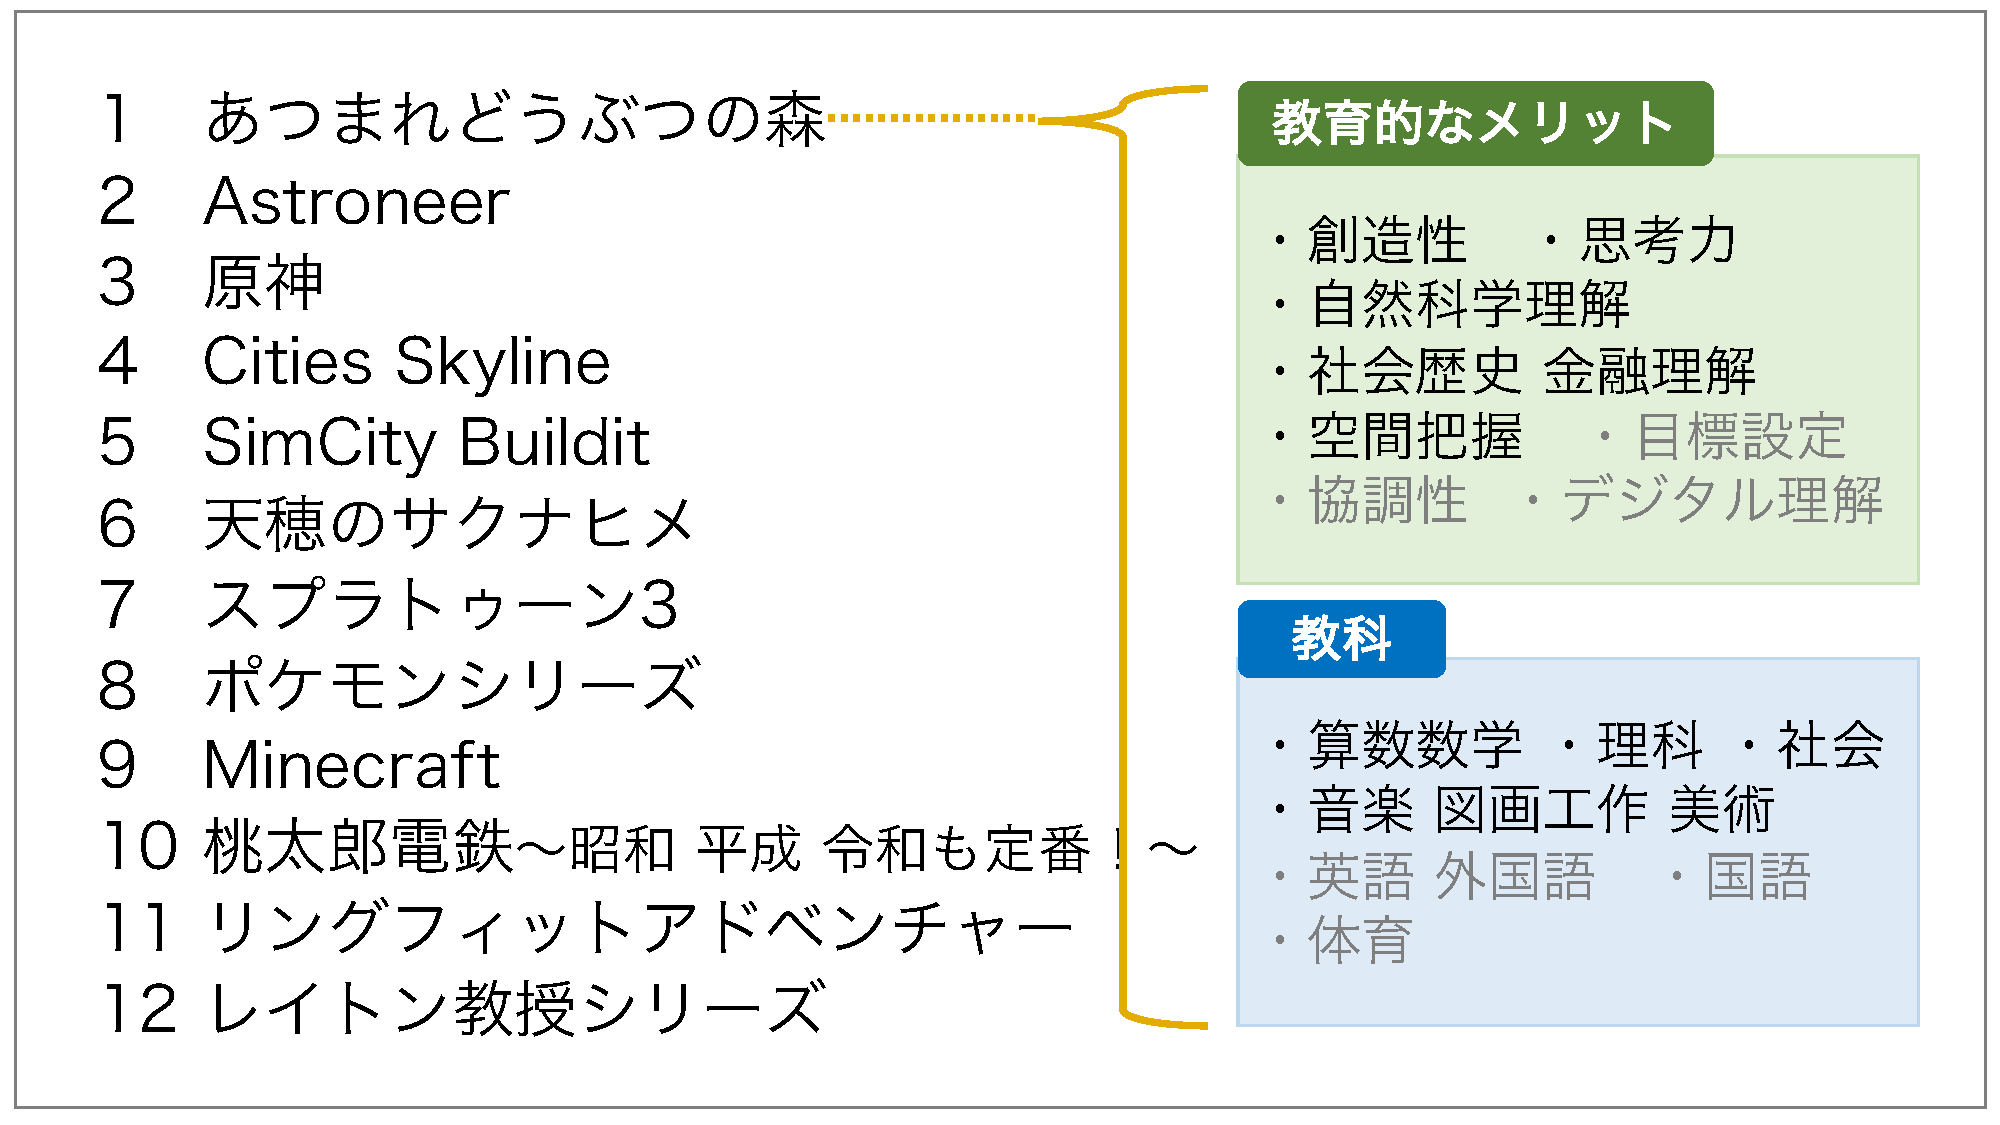
\includegraphics[clip,width=95mm,height=55mm]{games.pdf}
 \end{center}
 \caption{ゲーム一覧と「あつまれどうぶつの森」のタグ付け例}
 \label{fig:ゲーム一覧}
\end{figure}

\section{Webサイトとアンケートについて}
本研究では教育効果の明示による印象の変化を調査するため, Webサイトに掲載する娯楽ゲームは小中学生を対象にしたものに設定し,アンケートの対象者は小中学生の子を持つ保護者に設定した.
教育的メリットや教科は以下の図\ref{fig:ゲーム一覧}の右側ように設定し,紹介したゲームは左側の12個で右側の黒字部分は「あつまれどうぶつの森」にタグ付けした一例である.
記事の内容には紹介した娯楽ゲームの概要とタグ付けしたそれぞれの教育的なメリットについての説明をゲームの内容に沿って記述した.

アンケートは子の年齢やゲームのプレイ頻度,好き嫌い等の質問と,表\ref{table:SpeedOfLight}の項目を見る前と見た後について質問した.

\vspace{1zh}
\begin{table}[h]
 \caption{アンケート}
 \label{table:SpeedOfLight}
 \centering
  \begin{tabular}{l}
  \hline
  子に与える影響について \\
   \hline \hline
   発育・成長 \\
   勉強面 \\
   友人関係,コミュニケーション \\
   感性 \\
   知識,教養   \\
   時間管理 \\
   健康面 \\
   読書・スポーツ等他の趣味とのメリットの比較 \\
   \hline
  \end{tabular}
\end{table}


%\section{Webサイト制作と評価方法}
%掲載するエンターテイメントゲームは様々な種類のものを用意し,それぞれのゲームの種類やプレイによって得られるだろう教育的メリットでジャンル分けしタグ付けを行う.タグは,創造性,協調性,社会理解,デジタル理解,自然理解などの他,ワード検索もできるようにする予定である.またタグの他に,授業の教科に関連付けを行い教科からも検索できるようにする.図\ref{fig:スクショ}のゲームの詳細ページを示す.①の部分は検索機能でタグやキーワードから検索ができる欄である.②の部分はゲームのスクリーンショットとゲームプレイによって得ることが期待される教育的メリットについての詳細や具体例を記述する.

%評価にはアンケート調査で行う.対象者は小中学生の子を持つ保護者で,マーク形式で作成し,最後に自由記述欄を設ける.


%3章には,最終審査用の梗概では,やったことを示す.
%コンテンツを作成した場合にはコンテンツのスクリーンショットなどを用いる.
%調査が主であれば,調査の概要と結果のグラフなどを使用する.

%この文章では1章が長すぎるので,見た目のバランスが悪い.
%通常の梗概の割合は左側に1章と2章,右側に3章と4章のように並ぶ.
%もちろん多少の前後は有るので,きっちりと合わせなくても良い.

%通常,図は2枚程度である.
%図1枚+表1面でも構わない.
%梗概を書き始める前に,使用する図を決めてからレイアウトしていくと雰囲気がつかみやすくて良い.


\section{おわりに}
本研究では娯楽ゲームの印象改善を図るためのWebサイトを作成しアンケートによって良い印象に変わったという評価が得られた.
%今後はこのような娯楽ゲームのメリットが広く認知され,記述や教育の発展に繋げられることを期待している.
ただゲームの説明文がゲームをあまりしない人にとっては内容が想像しにくい点や教育効果の根拠が薄い点があるため,今後は記事内容を研鑽し共感を得られるものにすることが望まれる.

%中間審査用の梗概では4章のタイトルとして「今後の予定」,最終審査用の梗概では「おわりに」などを用いる.
%たいてい2〜3行程度でまとめる.

\begin{thebibliography}{99}
\bibitem{gameanq} ASMARQ : ``ゲームと子どもに関するアンケート調査'', \url{https://www.asmarq.co.jp/data/mr201409game/}, 2022/8/19参照
\bibitem{tvgame} 坂元 章 : ``21世紀はテレビゲーミング社会 ―娯楽主導から有効利用ヘ―'', 特定非営利活動法人日本シミュレーション&ゲーミング学会, 2000年 10 巻 1 号 p.4-13, 2000.
\end{thebibliography}

\end{document}
